\documentclass[12pt]{ctexart}
\usepackage{amsmath,amssymb,amsthm}
\usepackage{graphicx}
\usepackage{booktabs}
\usepackage{float}
\usepackage[table]{xcolor}
\usepackage{geometry}
\usepackage{caption}
\usepackage{multirow}
\usepackage{enumitem}
\usepackage{array}
\geometry{a4paper,margin=2.5cm}
\usepackage[colorlinks=true,allcolors=black]{hyperref}

\captionsetup{font=small,labelfont=bf}
\setlength{\parindent}{2em}

\title{\heiti 多波束测线问题的建模与优化}
\author{}
\date{}

\begin{document}

\maketitle
\vspace{-3em}
\begin{center}
\large\bfseries 摘要
\end{center}

多波束测深系统在与航迹垂直的平面内发射扇形波束，实现对海底的全覆盖扫描，测线设计的核心是覆盖宽度与相邻条带重叠率的控制。本文针对海底地形从平坦、倾斜到真实离散地形的递进场景，建立覆盖宽度的统一几何模型，并采用``简单基准模型＋针对性改进模型''的双模型策略逐步求解。

\textbf{针对问题一}，以平坦海底公式 $W=2D\tan(\theta/2)$ 为基准，建立射线—斜面求交模型刻画坡度影响，导出覆盖宽度解析式。在开角 $\theta=120^\circ$、坡度 $\alpha=1.5^\circ$、中心水深 $70\,\mathrm{m}$ 下，覆盖宽度由浅水侧 $170.27\,\mathrm{m}$ 单调增至深水侧 $315.71\,\mathrm{m}$；固定 $200\,\mathrm{m}$ 间距时重叠率由 $-11.51\%$（漏测）升至 $34.77\%$（冗余）。

\textbf{针对问题二}，将模型推广到测线方向与坡面法向水平投影成任意夹角 $\beta$，引入视坡度 $\tan\alpha_{\mathrm{eff}}=\tan\alpha|\sin\beta|$ 与位置相关水深，以统一公式覆盖全部 $8$ 个夹角与 $8$ 个距离的组合，问题一恰为 $\beta=90^\circ$ 的特例。

\textbf{针对问题三}，以平均水深等间距法与最浅处等间距法为双基准（分别仅 $23$ 条却漏测 $618\%$、需 $194$ 条却冗余 $94.7\%$），提出变间距贪心布设，利用覆盖宽度沿坡度方向的单调性证明其全局最优，得到\textbf{最少 $34$ 条测线、总长 $68$ 海里}，重叠率严格落在 $10\%$ 且完全覆盖。

\textbf{针对问题四}，基于附件 $251\times201$ 深度数据，经坡度主方向分析确定测线沿南北向，逐点计算覆盖宽度并做变间距布设。通过对间距系数做 $8$ 点扫描刻画``总长度—漏测—重叠''的三目标权衡，选定平衡方案：\textbf{测线 $49$ 条、总长 $245$ 海里、漏测面积占比 $4.21\%$、重叠率超 $20\%$ 部分总长 $94.8$ 海里}。

\medskip
\noindent\textbf{关键词：}多波束测深；覆盖宽度；视坡度；重叠率；测线优化；双模型对比

\newpage
\section{问题重述}

多波束测深是利用声波在水中的反射原理获取海底地形的重要手段\cite{li,zhao}。多波束测深系统在与航迹垂直的平面内一次发射数十至上百个波束，在海底平坦时能测得以测线为轴、宽度为 $W$ 的覆盖条带。换能器开角为 $\theta$，水深为 $D$。相邻测线间距为 $d$ 时，重叠率定义为
\begin{equation}
\eta=1-\frac{d}{W},
\end{equation}
$\eta<0$ 表示漏测。为保证测量质量与效率，相邻条带重叠率宜控制在 $10\%\sim20\%$。

真实海底地形起伏，若按海区平均水深设计等间距测线，水深较浅处会漏测；若按最浅处水深设计，水深较深处又重叠过多、数据冗余。本题需依次解决四个问题：建立坡度 $\alpha$ 下覆盖宽度与重叠率模型；建立任意夹角 $\beta$ 下的覆盖宽度模型；在均匀斜面海域设计最短测线；基于真实海底数据设计测线并计算三个指标。

\section{问题分析}

\textbf{问题的几何本质}是多波束扇形平面与海底曲面的求交。覆盖宽度由两个因素决定：该处\textbf{水深} $D$（近似线性影响）与垂直剖面内的\textbf{视坡度}（使覆盖宽度左右不对称，坡下侧展宽、坡上侧收窄）。

四个问题呈递进关系：问题一在二维剖面内建立基本求交模型；问题二将坡度方向与测线方向解耦，引入视坡度与位置相关水深；问题三在均匀斜面下利用单调性给出可证明最优的测线设计；问题四在真实离散地形上，将覆盖宽度视为随纵向位置变化的函数，转化为多目标优化。

依照``简单基准＋改进模型''的思路，每个问题都先以简化模型给出可对照的基准解，再引入针对该问关键因素的改进模型，通过对比证明改进的必要性与有效性，避免``为复杂而复杂''。具体而言，问题一以平坦海底公式为基准、以坡度下的射线—斜面求交为改进；问题二以沿等高线的特例为基准、以视坡度模型为改进；问题三以平均水深与最浅处两种等间距法为基准、以变间距贪心为改进；问题四以三种间距策略对比呈现 Pareto 权衡。每个改进模型的引入都有明确的问题动机，结论的可信度建立在可验证的定量对比之上。

总体技术路线为：首先建立覆盖宽度与重叠率的统一几何模型（问题一、二），然后以该模型为基础，分别在均匀斜面与真实地形上做测线优化（问题三、四），其中均匀斜面可解析求解并证明最优，真实地形则转为多目标权衡，最终形成从几何建模到优化设计的完整闭环。

\section{模型假设与符号说明}

\subsection{模型假设}
\begin{enumerate}[label=(\arabic*)]
\item 声波在海水介质中沿直线传播，忽略声速剖面引起的声线弯曲；
\item 换能器开角 $\theta$ 在测量过程中恒定，波束在垂直剖面内对称分布；
\item 在覆盖宽度尺度内，海底可视为局部平面（问题四的网格步长 $0.02$ 海里远小于地形水平变化尺度）；
\item 测量船沿测线匀速直线航行，测线为水平面内的直线。
\end{enumerate}

上述假设均有明确的适用范围。假设(3)的合理性可由数据尺度验证：附件网格步长 $0.02$ 海里（约 $37\,\mathrm{m}$），而覆盖宽度普遍在 $100\sim700\,\mathrm{m}$ 量级，覆盖宽度远大于网格步长，故在覆盖宽度尺度内海底可近似为局部平面，由局部坡度代入式(5)计算覆盖宽度是合理的近似。假设(1)忽略声线弯曲，本题水深均小于 $200\,\mathrm{m}$，在浅水区声速随深度变化引起的声线弯曲可忽略，该假设成立。本文使用的主要符号见表 \ref{tab:sym}。

\subsection{符号说明}
\begin{table}[H]\centering
\caption{主要符号说明}
\label{tab:sym}
\begin{tabular}{cl}
\toprule
符号 & 含义 \\
\midrule
$\theta$ & 多波束换能器开角 \\
$\alpha$ & 海底坡度（坡面与水平面夹角） \\
$\alpha_{\mathrm{eff}}$ & 垂直于测线剖面内的视坡度 \\
$\beta$ & 测线方向与坡面法向水平投影的夹角 \\
$D,\ D_0$ & 海水深度、海域中心点水深 \\
$W$ & 条带覆盖宽度 \\
$w_{\mathrm{shallow}},\ w_{\mathrm{deep}}$ & 坡上侧、坡下侧覆盖半宽 \\
$d$ & 相邻测线间距 \\
$\eta$ & 相邻条带重叠率 \\
$s$ & 测量船距海域中心点距离 \\
\bottomrule
\end{tabular}
\end{table}

\section{问题一：覆盖宽度与重叠率的数学模型}

\subsection{基准模型：平坦海底}

当海底水平（$\alpha=0$）时，左右波束对称打到海底，覆盖宽度由简单的三角关系给出
\begin{equation}
W_0 = 2D\tan\frac{\theta}{2}.
\end{equation}
该式是后续所有模型的退化基准，也是检验改进模型正确性的标尺。

\subsection{改进模型：坡度下的射线—斜面求交}

当海底坡面与水平面夹角为 $\alpha$ 且测线沿等高线时，垂直于测线的竖直平面与坡面的交线是一条倾角为 $\alpha$ 的斜线。以换能器为原点、竖直向下为 $z$ 轴正向，中心点水深 $D$，坡面在剖面内满足 $z=D+u\tan\alpha$，其中 $u$ 为剖面内水平坐标、向坡下为正。波束自换能器沿与竖直方向成角 $\varphi$ 的方向直线传播，其射线满足 $z=u\cot\varphi$。将其代入坡面方程 $z=D+u\tan\alpha$，得
\begin{equation}
u\cot\varphi=D+u\tan\alpha\ \Longrightarrow\ u(\cot\varphi-\tan\alpha)=D,
\end{equation}
整理为交点水平坐标
\begin{equation}
u(\varphi)=\frac{D}{\cot\varphi-\tan\alpha}=\frac{D\sin\varphi}{\cos\varphi-\sin\varphi\tan\alpha}.
\end{equation}
式(4)的几何含义清晰：分母 $\cos\varphi-\sin\varphi\tan\alpha$ 刻画了坡面对波束``落点''的推移作用。当 $\varphi$ 指向坡下（$\varphi>0$）时分母变小、半宽增大；指向坡上（$\varphi<0$）时分母变大、半宽减小，从而自然产生了覆盖宽度的不对称。
取左右最外侧波束 $\varphi=\pm\theta/2$，覆盖半宽分别为坡下侧与坡上侧：
\begin{equation}
w_{\mathrm{deep}}=\frac{D\sin\frac{\theta}{2}}{\cos\frac{\theta}{2}-\sin\frac{\theta}{2}\tan\alpha},\qquad
w_{\mathrm{shallow}}=\frac{D\sin\frac{\theta}{2}}{\cos\frac{\theta}{2}+\sin\frac{\theta}{2}\tan\alpha}.
\end{equation}
覆盖宽度为两者之和
\begin{equation}
\boxed{W=D\sin\frac{\theta}{2}\left[\frac{1}{\cos\frac{\theta}{2}-\sin\frac{\theta}{2}\tan\alpha}
+\frac{1}{\cos\frac{\theta}{2}+\sin\frac{\theta}{2}\tan\alpha}\right]}.
\end{equation}
当 $\alpha=0$ 时，式(5)退化为 $W=2D\tan(\theta/2)$，与基准模型一致，验证了模型正确性。

\subsection{模型对比与坡度灵敏度}

在 $D=70\,\mathrm{m}$ 处计算不同坡度下的覆盖宽度，见表 \ref{tab:p1sens}。

\begin{table}[H]\centering
\caption{坡度对覆盖宽度的影响（$D=70\,\mathrm{m}$）}
\label{tab:p1sens}
\begin{tabular}{ccccccc}
\toprule
坡度 $\alpha$ /° & 0 & 0.5 & 1 & 1.5 & 2 & 3 \\
\midrule
覆盖宽度 /m & 242.49 & 242.54 & 242.71 & 242.99 & 243.38 & 244.50 \\
相对平坦变化 /\% & 0.00 & 0.02 & 0.09 & 0.21 & 0.37 & 0.83 \\
\bottomrule
\end{tabular}
\end{table}

表 \ref{tab:p1sens} 表明，在本题参数范围内坡度对\textbf{总覆盖宽度}的影响很小（$1.5^\circ$ 时仅 $+0.21\%$），原因在于 $\tan\alpha\ll\cot(\theta/2)$。然而坡度模型的实质贡献不在总宽度，而在\textbf{左右不对称}：坡下侧半宽 $w_{\mathrm{deep}}=127.0\,\mathrm{m}$、坡上侧半宽 $w_{\mathrm{shallow}}=116.0\,\mathrm{m}$，两者相差 $11\,\mathrm{m}$，不对称度约 $4.5\%$。这一不对称正是重叠率计算的本质——相邻条带的重叠发生在一条测线的坡下侧与另一条测线的坡上侧之间，忽略不对称会低估浅水侧漏测风险。

为进一步考察水深与坡度的联合影响，绘制覆盖宽度 $W(D,\alpha)$ 的等高线图，见图 \ref{fig:p1wda}。

\begin{figure}[H]\centering
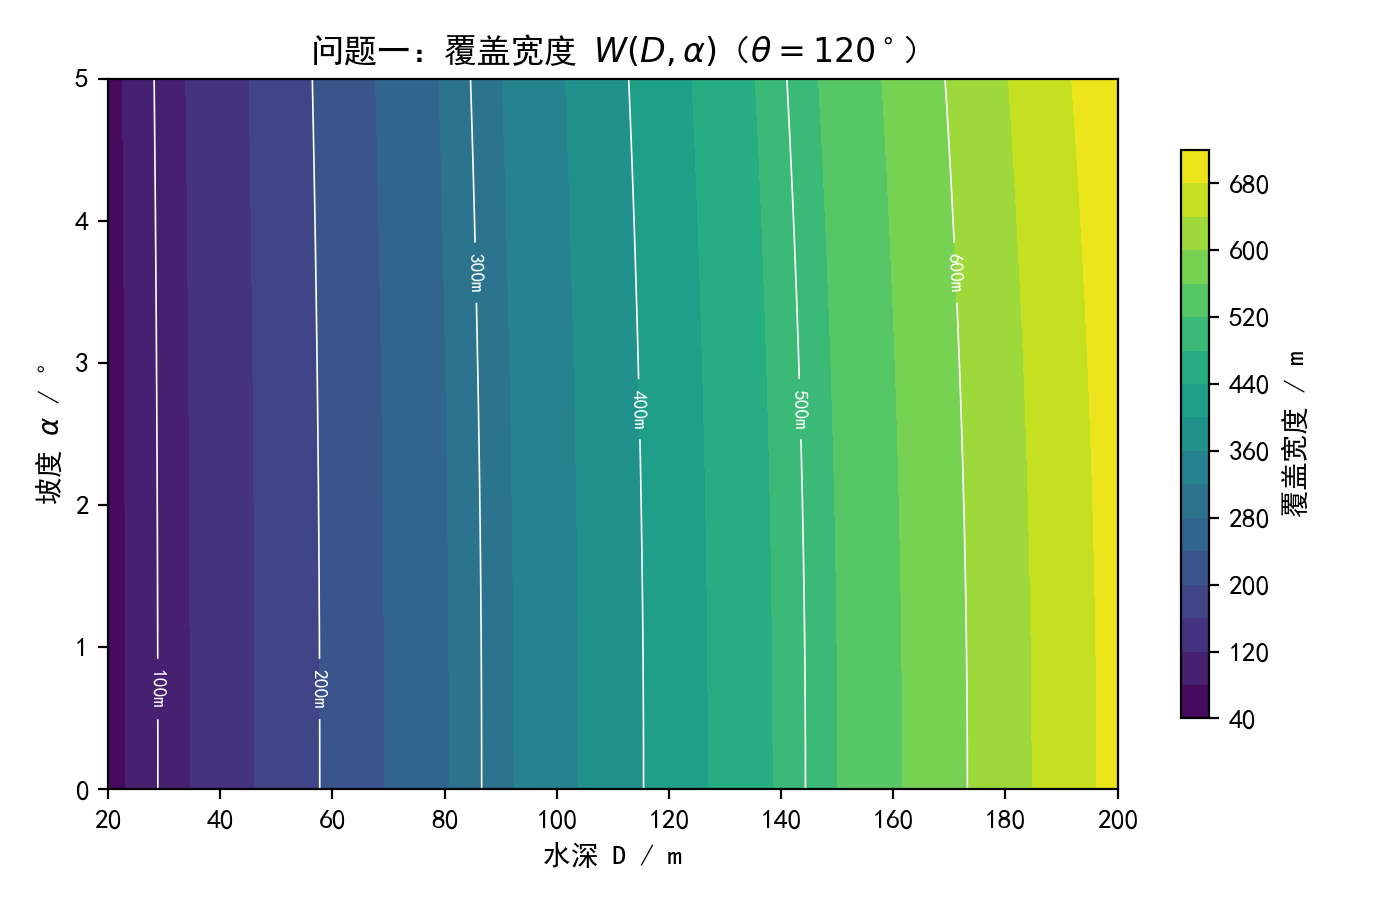
\includegraphics[width=0.68\textwidth]{output/figures/fig_p1_WDa.png}
\caption{问题一：覆盖宽度 $W(D,\alpha)$ 的等高线图（$\theta=120^\circ$）}
\label{fig:p1wda}
\end{figure}

图 \ref{fig:p1wda} 的等高线近似为等间距的竖直直线，表明覆盖宽度对水深呈近似线性依赖（$W\propto D$）；而沿 $\alpha$ 方向等高线几乎水平，表明覆盖宽度对坡度不敏感。这两点与式(5)的结构完全一致：$W$ 的主项 $2D\tan(\theta/2)$ 正比于 $D$，坡度项为 $O(\tan^2\alpha)$ 的小量修正，只有当坡度较大时才不可忽略。

\subsection{重叠率模型与计算结果}

相邻测线间距为 $d$ 时，由于覆盖宽度随水深变化，取相邻两条测线覆盖宽度的平均值 $\overline{W}=(W_{i-1}+W_i)/2$ 为重叠率基准，得
\begin{equation}
\eta_i=1-\frac{2d}{W_{i-1}+W_i}.
\end{equation}
测线距中心点距离为 $x$（向东为坡下）时，水深 $D(x)=D_0+x\tan\alpha$，$D_0=70\,\mathrm{m}$。计算结果见表 \ref{tab:p1}。

\begin{table}[H]\centering
\caption{问题一计算结果（$\theta=120^\circ,\ \alpha=1.5^\circ,\ D_0=70\,\mathrm{m}$）}
\label{tab:p1}
\footnotesize
\resizebox{\textwidth}{!}{%
\begin{tabular}{cccccccccc}
\toprule
距中心点距离/m & $-800$ & $-600$ & $-400$ & $-200$ & $0$ & $200$ & $400$ & $600$ & $800$ \\
\midrule
海水深度/m & 49.05 & 54.29 & 59.53 & 64.76 & 70.00 & 75.24 & 80.47 & 85.71 & 90.95 \\
覆盖宽度/m & 170.27 & 188.45 & 206.63 & 224.81 & 242.99 & 261.17 & 279.35 & 297.53 & 315.71 \\
与前一条重叠率/\% & — & $-11.51$ & $-1.25$ & 7.29 & 14.49 & 20.66 & 26.00 & 30.66 & 34.77 \\
\bottomrule
\end{tabular}}
\end{table}

\begin{figure}[H]\centering
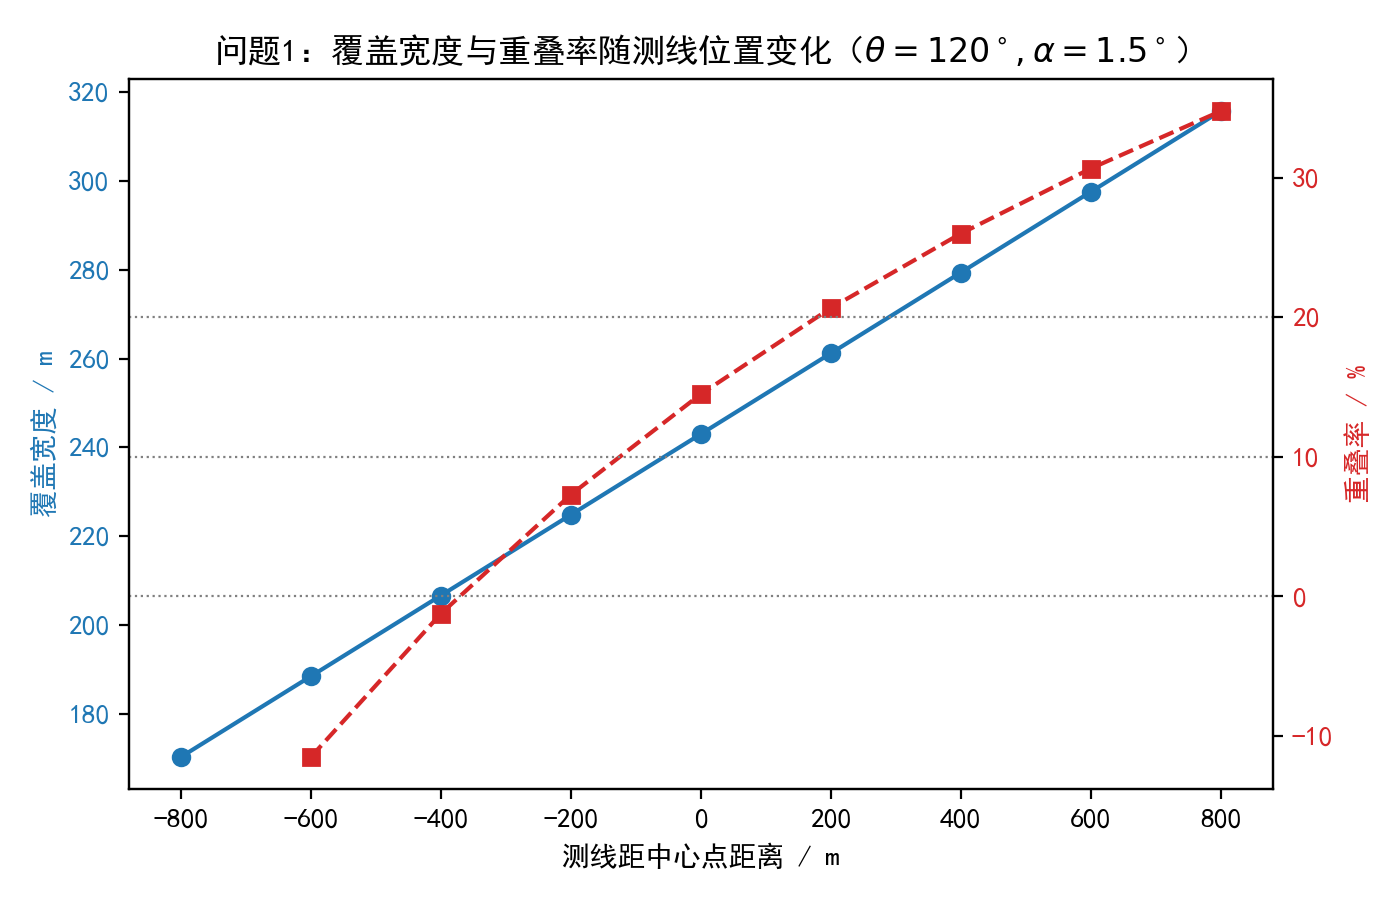
\includegraphics[width=0.72\textwidth]{output/figures/fig_p1.png}
\caption{问题一：覆盖宽度与重叠率随测线位置的变化（虚线为 $0\%$、$10\%$、$20\%$ 参考线）}
\label{fig:p1}
\end{figure}

由图 \ref{fig:p1} 与表 \ref{tab:p1} 可见三点规律：其一，覆盖宽度随水深由 $170.27\,\mathrm{m}$ 单调增至 $315.71\,\mathrm{m}$，与式(5)的线性依赖一致；其二，固定 $200\,\mathrm{m}$ 间距时重叠率由浅水侧的 $-11.51\%$（漏测）单调升至深水侧的 $34.77\%$（重叠过多）；其三，仅当测线距中心点约 $0\sim200\,\mathrm{m}$ 附近，重叠率才落在理想的 $10\%\sim20\%$ 区间内。这定量地印证了题述``平均间距漏测、最浅处间距冗余''的矛盾，为问题三的变间距设计埋下伏笔。

\section{问题二：任意测线方向下的覆盖宽度}

\subsection{基准模型：沿等高线的特例}

当测线沿等高线（$\beta=90^\circ$）时，垂直剖面内看到完整坡度 $\alpha$，覆盖宽度即问题一的式(5)，且移动测量船不改变水深，覆盖宽度恒为常数。这是问题二最简情形，作为基准。

\subsection{改进模型：视坡度与位置相关水深}

当测线方向与坡面法向水平投影成任意夹角 $\beta$ 时，需要引入两个修正。

\textbf{(1) 视坡度。}垂直于测线的剖面不再沿最陡方向，坡面在该剖面内的视坡度满足
\begin{equation}
\tan\alpha_{\mathrm{eff}}=\tan\alpha\,|\sin\beta|.
\end{equation}
$\beta=90^\circ$ 时 $\alpha_{\mathrm{eff}}=\alpha$（退化到基准），$\beta=0^\circ$ 时 $\alpha_{\mathrm{eff}}=0$（剖面内海底水平）。

这一关系的严格推导如下。设坡面法向在水平面的投影方向（上坡方向）为单位向量 $\boldsymbol{e}$，测线方向的单位向量为 $\boldsymbol{t}$，二者夹角为 $\beta$；垂直于测线的水平方向单位向量为 $\boldsymbol{u}$，其与 $\boldsymbol{e}$ 的夹角为 $90^\circ-\beta$。坡面梯度水平分量的大小为 $\tan\alpha$、方向为 $\boldsymbol{e}$，故剖面内（沿 $\boldsymbol{u}$ 方向）海底坡面的视坡度为
\begin{equation}
\tan\alpha_{\mathrm{eff}}=\left|\nabla z\cdot\boldsymbol{u}\right|=\tan\alpha\,|\boldsymbol{e}\cdot\boldsymbol{u}|=\tan\alpha\,|\sin\beta|.
\end{equation}
这一推导表明，视坡度本质上是真实坡度在垂直于测线方向上的投影，当测线恰好沿等高线（$\beta=90^\circ$）时投影取最大值 $\tan\alpha$。

\textbf{(2) 位置相关水深。}测量船沿测线方向偏离中心点 $s$（海里）时，位移在坡面下降方向的投影引起水深变化：
\begin{equation}
D(s,\beta)=D_0-s\cos\beta\cdot\tan\alpha\cdot1852.
\end{equation}
$\beta=90^\circ$ 时移动不改变水深，$\beta=0^\circ$（沿上坡）时水深随 $s$ 减小最快。

将式(7)的视坡度与式(8)的水深代入式(5)，得覆盖宽度的统一表达式
\begin{equation}
W(\beta,s)=D(s,\beta)\sin\frac{\theta}{2}\left[\frac{1}{\cos\frac{\theta}{2}-\sin\frac{\theta}{2}\tan\alpha_{\mathrm{eff}}}
+\frac{1}{\cos\frac{\theta}{2}+\sin\frac{\theta}{2}\tan\alpha_{\mathrm{eff}}}\right].
\end{equation}

\subsection{计算结果与分析}

取 $D_0=120\,\mathrm{m}$、$\alpha=1.5^\circ$、$\theta=120^\circ$，对 $\beta\in\{0^\circ,45^\circ,\dots,315^\circ\}$ 与 $s\in\{0,0.3,\dots,2.1\}$ 海里逐点计算，结果见表 \ref{tab:p2} 与图 \ref{fig:p2}。

\begin{table}[H]\centering
\caption{问题二覆盖宽度 $W$（单位：m）}
\label{tab:p2}
\small
\begin{tabular}{ccccccccc}
\toprule
$\beta/$° & \multicolumn{8}{c}{测量船距中心点距离 /海里} \\
 & 0 & 0.3 & 0.6 & 0.9 & 1.2 & 1.5 & 1.8 & 2.1 \\
\midrule
0 & 415.69 & 365.29 & 314.89 & 264.50 & 214.10 & 163.70 & 113.30 & 62.90 \\
45 & 416.12 & 380.45 & 344.77 & 309.10 & 273.42 & 237.75 & 202.08 & 166.40 \\
90 & 416.55 & 416.55 & 416.55 & 416.55 & 416.55 & 416.55 & 416.55 & 416.55 \\
135 & 416.12 & 451.79 & 487.47 & 523.14 & 558.82 & 594.49 & 630.16 & 665.84 \\
180 & 415.69 & 466.09 & 516.49 & 566.89 & 617.29 & 667.69 & 718.09 & 768.48 \\
225 & 416.12 & 451.79 & 487.47 & 523.14 & 558.82 & 594.49 & 630.16 & 665.84 \\
270 & 416.55 & 416.55 & 416.55 & 416.55 & 416.55 & 416.55 & 416.55 & 416.55 \\
315 & 416.12 & 380.45 & 344.77 & 309.10 & 273.42 & 237.75 & 202.08 & 166.40 \\
\bottomrule
\end{tabular}
\end{table}

\begin{figure}[H]\centering
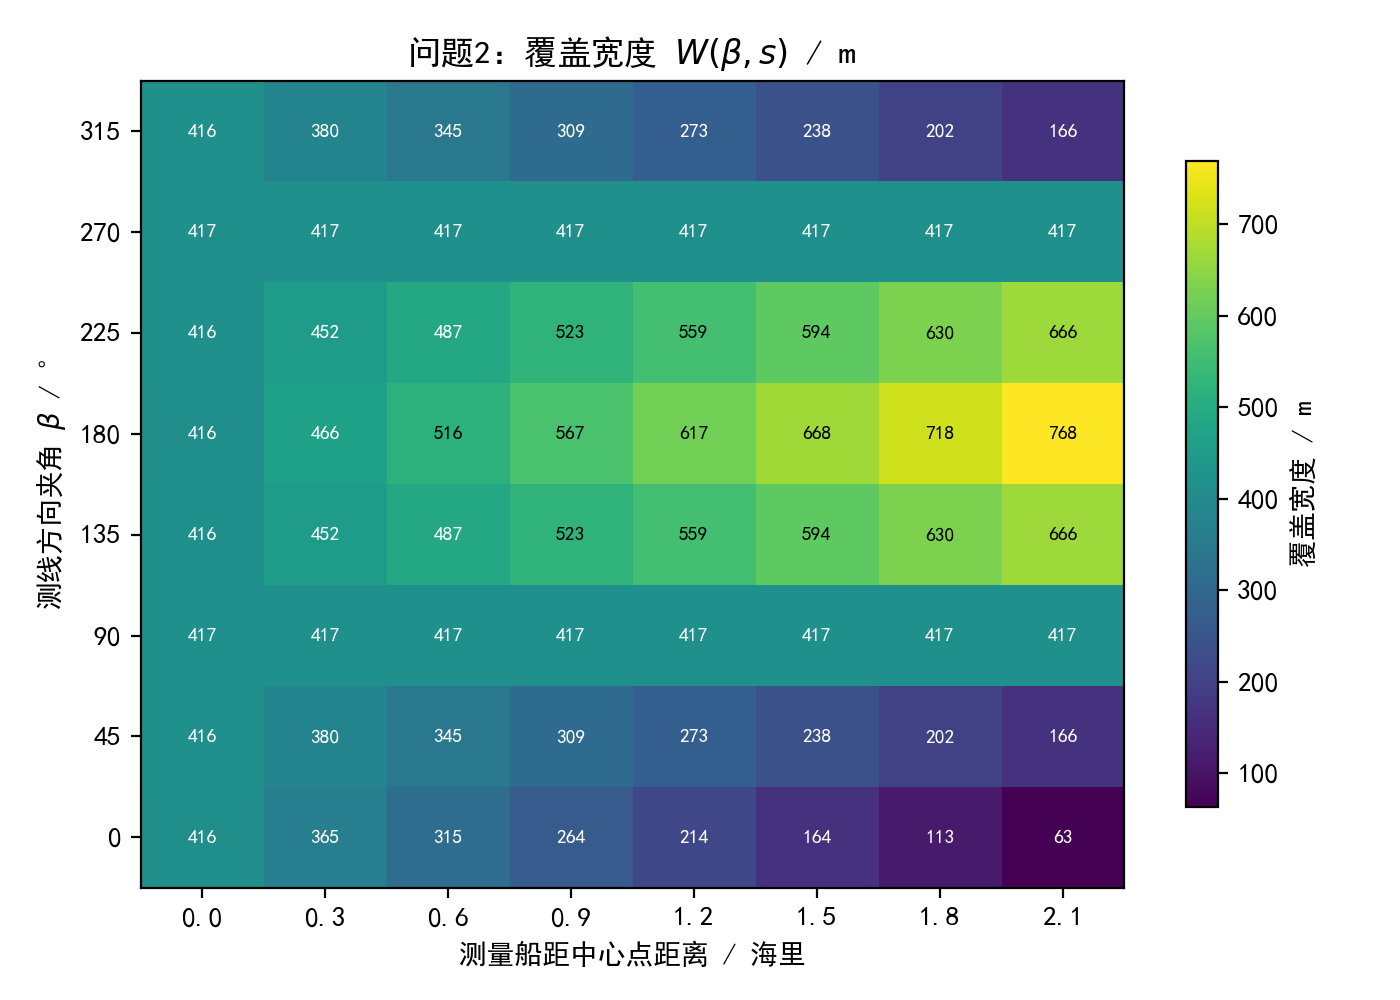
\includegraphics[width=0.72\textwidth]{output/figures/fig_p2.png}
\caption{问题二：覆盖宽度随夹角 $\beta$ 与距离 $s$ 的分布}
\label{fig:p2}
\end{figure}

表 \ref{tab:p2} 与图 \ref{fig:p2} 呈现清晰的对称结构。其一，$\beta=90^\circ$ 与 $270^\circ$ 两行覆盖宽度恒为 $416.55\,\mathrm{m}$ 且不随 $s$ 变化，因为沿等高线移动水深不变，这与基准模型一致；其二，结果关于 $\beta=180^\circ$ 对称，即 $\beta$ 与 $360^\circ-\beta$ 的覆盖宽度相同；其三，$\beta=0^\circ$ 与 $180^\circ$ 分别对应沿上坡、下坡方向移动，覆盖宽度随 $s$ 单调减小、增大，二者在 $s=0$ 处均为 $415.69\,\mathrm{m}$ 且略小于 $\beta=90^\circ$ 的 $416.55\,\mathrm{m}$，差异来自视坡度由 $\tan\alpha$ 降为 $0$ 带来的微小变化。

为进一步揭示视坡度的作用机制，考察 $\tan\alpha_{\mathrm{eff}}=\tan\alpha|\sin\beta|$ 随 $\beta$ 的变化。当 $\beta=90^\circ$ 或 $270^\circ$ 时，$|\sin\beta|=1$，视坡度取最大值 $\tan\alpha$，覆盖宽度最大；当 $\beta=0^\circ$ 或 $180^\circ$ 时，$|\sin\beta|=0$，视坡度为零，剖面内海底水平，覆盖宽度回到平坦公式。因此覆盖宽度随 $|\sin\beta|$ 的增大而单调增大，这一规律在表 \ref{tab:p2} 的 $s=0$ 列得到验证（由 $415.69$ 增至 $416.55\,\mathrm{m}$）。与此同时，位置相关水深通过 $\cos\beta$ 项引入覆盖宽度随 $s$ 的线性变化：$|\cos\beta|$ 越大，测线方向越接近坡向，移动时水深变化越剧烈。视坡度与位置水深两项分别由 $\sin\beta$ 与 $\cos\beta$ 控制，二者相互独立、共同构成覆盖宽度随 $(\beta,s)$ 变化的完整图景。

为更完整地展示覆盖宽度随夹角的连续变化规律，在 $s=0$、$D_0=120\,\mathrm{m}$ 下对 $\beta\in[0^\circ,360^\circ]$ 做连续扫描，结果见图 \ref{fig:p2beta}。

\begin{figure}[H]\centering
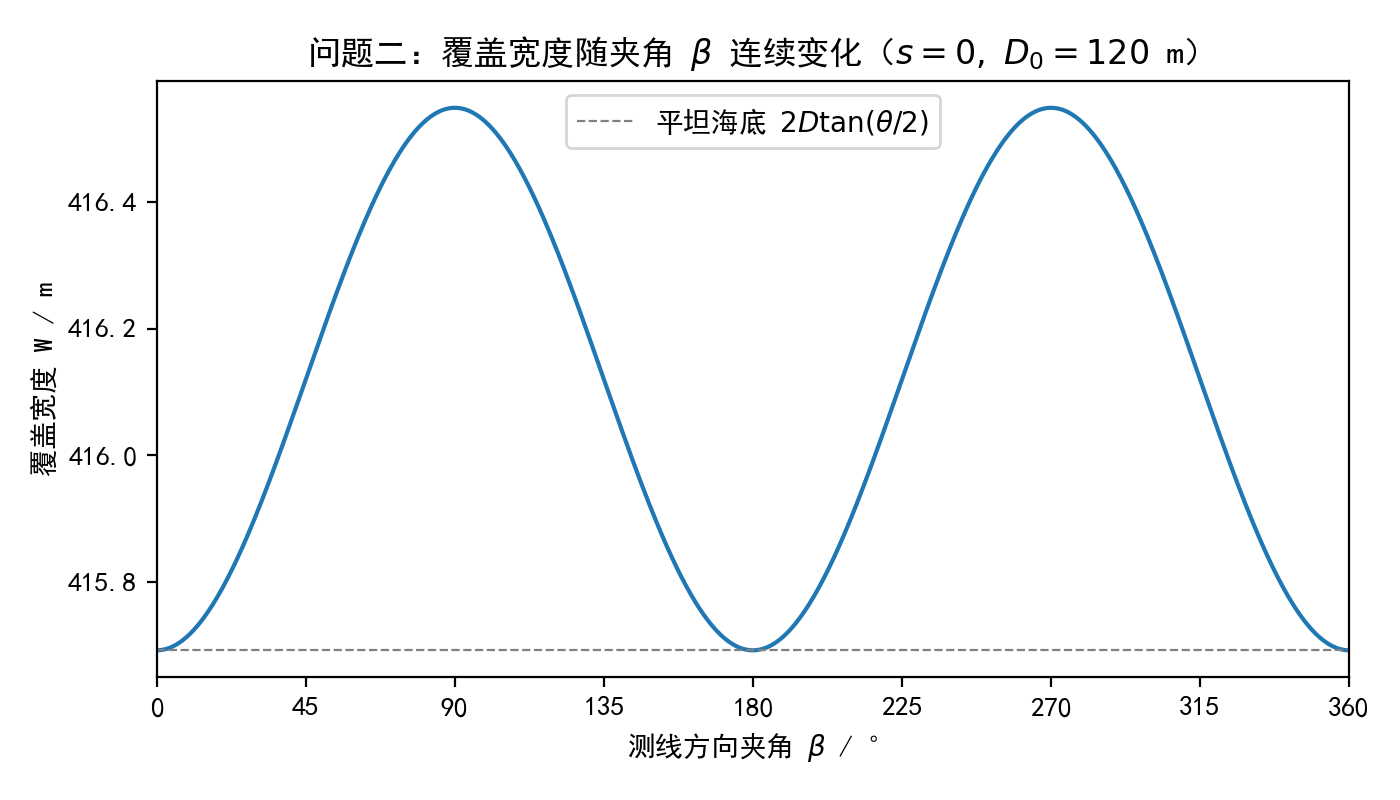
\includegraphics[width=0.68\textwidth]{output/figures/fig_p2_beta.png}
\caption{问题二：覆盖宽度随夹角 $\beta$ 连续变化（$s=0$，虚线为平坦海底基准）}
\label{fig:p2beta}
\end{figure}

图 \ref{fig:p2beta} 表明，覆盖宽度随 $\beta$ 以 $180^\circ$ 为周期变化，这是因为 $|\sin\beta|$ 的周期为 $180^\circ$。覆盖宽度在 $\beta=90^\circ,270^\circ$ 即沿等高线处取最大值 $416.55\,\mathrm{m}$，在 $\beta=0^\circ,180^\circ$ 即沿坡向处取最小值 $415.69\,\mathrm{m}$，二者仅相差 $0.86\,\mathrm{m}$，约为 $0.21\%$。这一微小差异再次印证了视坡度对总覆盖宽度的影响有限，其作用主要体现在覆盖宽度的左右不对称分布上。

\section{问题三：均匀斜面的最短测线设计}

\subsection{基准模型：两种等间距布设法}

海域东西向倾斜（西深东浅、坡度 $1.5^\circ$），等高线沿南北向。东西宽 $4$ 海里（$7408\,\mathrm{m}$），中心水深 $110\,\mathrm{m}$，东端水深仅 $13.0\,\mathrm{m}$、西端水深 $207.0\,\mathrm{m}$，覆盖宽度由东端 $45.2\,\mathrm{m}$ 到西端 $718.5\,\mathrm{m}$ 相差约 $16$ 倍。

\textbf{基准一（平均水深法）}：以中心水深 $110\,\mathrm{m}$ 的覆盖宽度 $W=381.8\,\mathrm{m}$ 为参考，取等间距 $d=0.85W=324.6\,\mathrm{m}$，需 $23$ 条测线。但在东端水深 $13\,\mathrm{m}$ 处覆盖宽度仅 $45.2\,\mathrm{m}$，远小于间距，重叠率低至 $-618.8\%$，即东半部约 $41\%$ 的海域严重漏测。

\textbf{基准二（最浅处法）}：以东端最浅处覆盖宽度 $45.2\,\mathrm{m}$ 为参考，取等间距 $d=38.4\,\mathrm{m}$，需 $194$ 条测线。但在西端深水处覆盖宽度达 $718.5\,\mathrm{m}$，重叠率高达 $94.7\%$，数据冗余极其严重。

上述两个基准分别对应题述图 5、图 6 的两种缺陷，二者都无法同时满足``完全覆盖＋重叠率 $10\%\sim20\%$''的要求。

\subsection{改进模型：变间距贪心布设}

\textbf{测线方向的最优性}：由式(7)，测线沿等高线（$\beta=90^\circ$）时视坡度最大、单线覆盖宽度最大，任意斜向测线都会因视坡度减小而降低覆盖效率，因此测线沿南北向布设最优。

设东西向坐标 $x$（中心为原点，向东为浅水），水深与覆盖宽度为
\begin{equation}
D(x)=D_0-x\tan\alpha,\qquad
W(x)=D(x)\sin\frac{\theta}{2}\left[\frac{1}{\cos\frac{\theta}{2}-\sin\frac{\theta}{2}\tan\alpha}+\frac{1}{\cos\frac{\theta}{2}+\sin\frac{\theta}{2}\tan\alpha}\right],
\end{equation}
其中 $D_0=110\,\mathrm{m}$，$x\in[-3704,3704]\,\mathrm{m}$。$W(x)$ 随 $x$ 向东单调递减。

要使总长度（正比于测线条数）最小，每条相邻间距应取\textbf{允许的最大值}，即重叠率取最小值 $10\%$。由于 $W(x)$ 单调，``每条测线取最大间距''的贪心布设即为全局最优：若某相邻间距小于最大允许值，将其增大既不违背重叠率下界（不漏测），又不增加测线数。这一结论可由区间覆盖问题的交换论证严格保证。

最少测线数的积分估计为
\begin{equation}
N^{*}=\left\lceil\int_{-3704}^{3704}\frac{\mathrm{d}x}{0.9\,W(x)}\right\rceil=\lceil 33.83\rceil=34.
\end{equation}
递推求解可概括为以下三步：

\textbf{第一步（初始化）}：解方程 $x_1-w_{\mathrm{deep}}(x_1)=-3704$，确定首条测线位置，使西侧覆盖边缘恰好落在西边界。由于 $w_{\mathrm{deep}}(x)$ 是 $x$ 的线性函数，该方程有唯一解析解。

\textbf{第二步（递推）}：设当前测线位置为 $x_i$，解方程
\begin{equation}
1-\frac{2(x_{i+1}-x_i)}{W(x_i)+W(x_{i+1})}=0.10
\end{equation}
求下一测线位置 $x_{i+1}$。由于 $W(x)$ 是 $x$ 的线性函数，上式是关于 $x_{i+1}$ 的一元二次方程，也可直接用二分法数值求解。

\textbf{第三步（终止）}：当 $x_{i+1}+w_{\mathrm{shallow}}(x_{i+1})\ge 3704$ 时停止，此时末条测线已覆盖东边界。

由于 $W(x)$ 单调，每步方程有唯一解，递推必然有限步终止，得到 $34$ 条测线，位置见表 \ref{tab:p3}，布设见图 \ref{fig:p3}。相邻测线间距沿东西方向的变化见图 \ref{fig:p3spacing}。

\begin{figure}[H]\centering
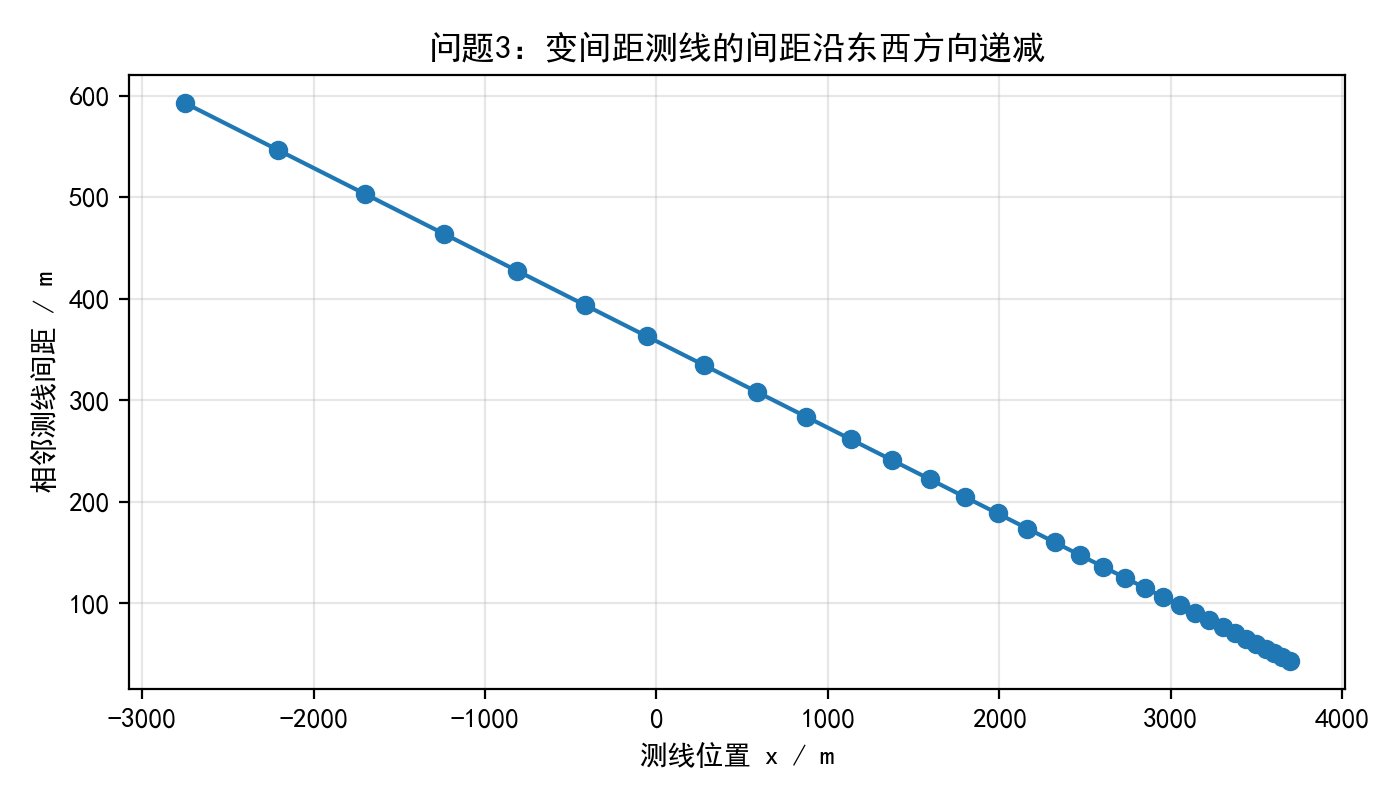
\includegraphics[width=0.7\textwidth]{output/figures/fig_p3_spacing.png}
\caption{问题三：变间距测线的相邻间距沿东西方向单调递减}
\label{fig:p3spacing}
\end{figure}

图 \ref{fig:p3spacing} 直观呈现了变间距策略的本质：间距由西端（深水）约 $593\,\mathrm{m}$ 单调递减至东端（浅水）约 $43\,\mathrm{m}$，恰好与覆盖宽度沿坡度方向的变化趋势一致，从而在每一处都维持 $10\%$ 的重叠率。

\begin{table}[H]\centering
\caption{问题三测线位置（东西向，单位：m）}
\label{tab:p3}
\small
\begin{minipage}[t]{0.45\textwidth}\centering
\begin{tabular}{rr}
\toprule
序号 & 位置/m \\
\midrule
1 & $-3345$ \\ 2 & $-2752$ \\ 3 & $-2206$ \\ 4 & $-1702$ \\
5 & $-1238$ \\ 6 & $-811$ \\ 7 & $-417$ \\ 8 & $-54$ \\
9 & $280$ \\ 10 & $588$ \\ 11 & $872$ \\ 12 & $1134$ \\
13 & $1375$ \\ 14 & $1597$ \\ 15 & $1802$ \\ 16 & $1990$ \\
17 & $2164$ \\
\bottomrule
\end{tabular}
\end{minipage}\hfill
\begin{minipage}[t]{0.45\textwidth}\centering
\begin{tabular}{rr}
\toprule
序号 & 位置/m \\
\midrule
18 & $2324$ \\ 19 & $2471$ \\ 20 & $2607$ \\ 21 & $2733$ \\
22 & $2848$ \\ 23 & $2954$ \\ 24 & $3052$ \\ 25 & $3143$ \\
26 & $3226$ \\ 27 & $3302$ \\ 28 & $3373$ \\ 29 & $3438$ \\
30 & $3498$ \\ 31 & $3553$ \\ 32 & $3604$ \\ 33 & $3651$ \\
34 & $3694$ \\
\bottomrule
\end{tabular}
\end{minipage}
\end{table}

\begin{figure}[H]\centering
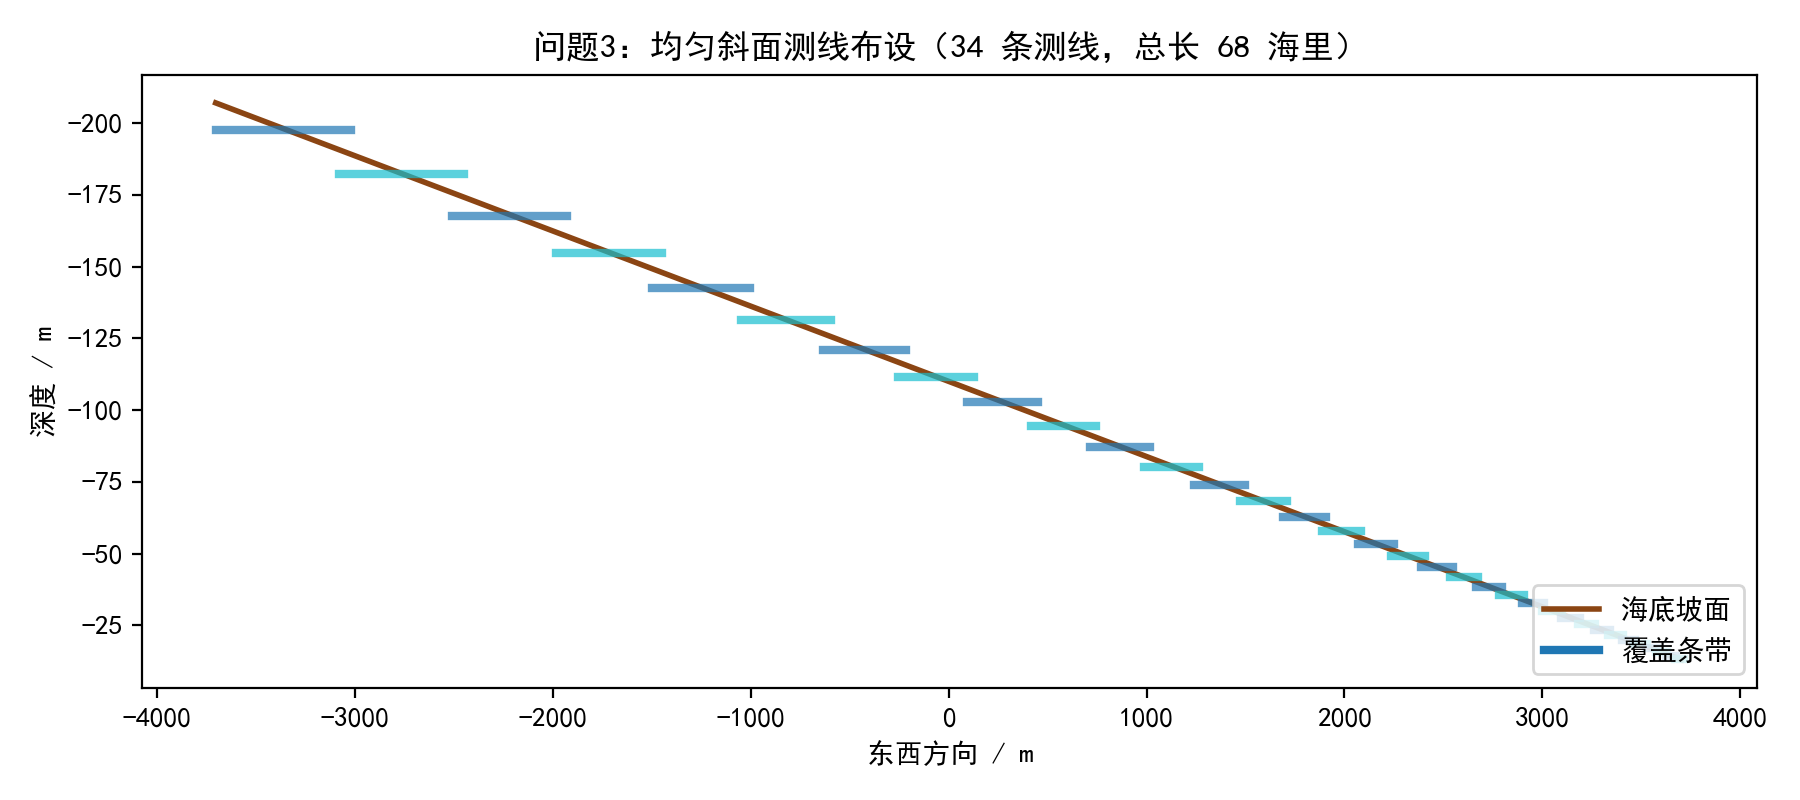
\includegraphics[width=0.85\textwidth]{output/figures/fig_p3.png}
\caption{问题三：均匀斜面测线布设（34 条，总长 68 海里，覆盖条带交替着色）}
\label{fig:p3}
\end{figure}

\subsection{模型对比}

三种布设方案的指标对比如表 \ref{tab:p3cmp}。

\begin{table}[H]\centering
\caption{问题三三种布设方案对比}
\label{tab:p3cmp}
\begin{tabular}{lccc}
\toprule
方案 & 测线数 & 总长度/海里 & 重叠率表现 \\
\midrule
平均水深等间距 & 23 & 46 & 东端漏测 $-618.8\%$ \\
最浅处等间距 & 194 & 388 & 西端冗余 $94.7\%$ \\
\textbf{变间距（本文）} & \textbf{34} & \textbf{68} & \textbf{全部 $10\%$，完全覆盖} \\
\bottomrule
\end{tabular}
\end{table}

表 \ref{tab:p3cmp} 显示，变间距方案以 $34$ 条测线同时实现了完全覆盖与重叠率 $10\%$，而两种等间距基准要么漏测要么冗余，鲜明体现了变间距策略的必要性：它依据覆盖宽度沿坡度方向的变化自适应地缩放间距，在深水区放大间距、浅水区缩小间距，从而以最少测线数兼顾覆盖完整性与重叠率约束。

经逐对验证，全部 $33$ 个相邻重叠率均为 $10.00\%$，东西边界分别被精确覆盖（西边界 $-3704.00\,\mathrm{m}$、东边界 $3716.15\,\mathrm{m}$）。

\subsection{重叠率下限的灵敏度}

题目要求重叠率在 $10\%\sim20\%$，其中下限 $10\%$ 决定测线数上限。改变重叠率下限 $\eta_{\min}$ 重算最少测线数，结果见表 \ref{tab:p3sens}。

\begin{table}[H]\centering
\caption{重叠率下限对最少测线数的影响}
\label{tab:p3sens}
\begin{tabular}{cccccc}
\toprule
重叠率下限 $\eta_{\min}$ /\% & 8 & 10 & 12 & 15 & 20 \\
\midrule
最少测线数 & 33 & 34 & 35 & 36 & 38 \\
总长度 /海里 & 66 & 68 & 70 & 72 & 76 \\
\bottomrule
\end{tabular}
\end{table}

表 \ref{tab:p3sens} 表明，重叠率下限每放宽 $2\sim5$ 个百分点，测线数仅减少 $1\sim2$ 条，测线数对重叠率下限不敏感，说明 $34$ 条的结论稳健。在满足题设 $10\%\sim20\%$ 的前提下，取最紧的下限 $10\%$ 即对应最少的 $34$ 条。

\section{问题四：真实海底地形的测线设计}

\subsection{数据特征与测线方向}

附件给出南北长 5 海里、东西宽 4 海里的海域，横向（西→东）$0\sim4$ 海里、纵向（南→北）$0\sim5$ 海里，网格步长 $0.02$ 海里，共 $251\times201$ 个测深点。由数值梯度计算深度场沿两方向的坡度，得到数据特征汇总于表 \ref{tab:data}。

\begin{table}[H]\centering
\caption{附件海底深度数据特征}
\label{tab:data}
\begin{tabular}{lcc}
\toprule
统计量 & 取值 & 说明 \\
\midrule
海域范围 & $4\times5$ 海里 & 东西 $\times$ 南北 \\
网格规模 & $201\times251$ & 横向 $\times$ 纵向，步长 $0.02$ 海里 \\
深度范围 & $20.0\sim197.2$ m & 均值 $62.5$ m \\
东西向坡度 $|\tan\alpha_x|$ & 平均 $0.011$、最大 $0.054$ & 约 $0.6^\circ$、最大 $3.1^\circ$ \\
南北向坡度 $|\tan\alpha_y|$ & 平均 $0.0066$、最大 $0.023$ & 约 $0.4^\circ$、最大 $1.3^\circ$ \\
\bottomrule
\end{tabular}
\end{table}

由表 \ref{tab:data} 可见，东西向平均坡度约为南北向的 $1.7$ 倍，地形主要沿东西向倾斜，等高线大致沿南北向，故测线沿南北方向布设。

\subsection{逐点覆盖宽度}

测线沿南北向时，垂直于测线的方向为东西向。在测线位置 $x$、纵向位置 $y$ 处，覆盖半宽由该点水深 $D(x,y)$ 与东西向局部坡度 $\tan\alpha_x=\left|\partial z/\partial x\right|$ 决定：
\begin{equation}
w_{\mathrm{deep}}(x,y)=\frac{D(x,y)\sin\frac{\theta}{2}}{\cos\frac{\theta}{2}-\sin\frac{\theta}{2}\tan\alpha_x},\quad
w_{\mathrm{shallow}}(x,y)=\frac{D(x,y)\sin\frac{\theta}{2}}{\cos\frac{\theta}{2}+\sin\frac{\theta}{2}\tan\alpha_x}.
\end{equation}
坡下方向由 $\partial z/\partial x$ 的符号确定，从而得到测线两侧的非对称覆盖区间。由于水深沿南北向起伏（南端浅水约 $20\,\mathrm{m}$、北端深水），覆盖宽度随 $y$ 显著变化，单一间距无法同时满足所有纬度处的重叠要求，这正是真实地形测线设计相较问题三的难点所在。

\begin{figure}[H]\centering
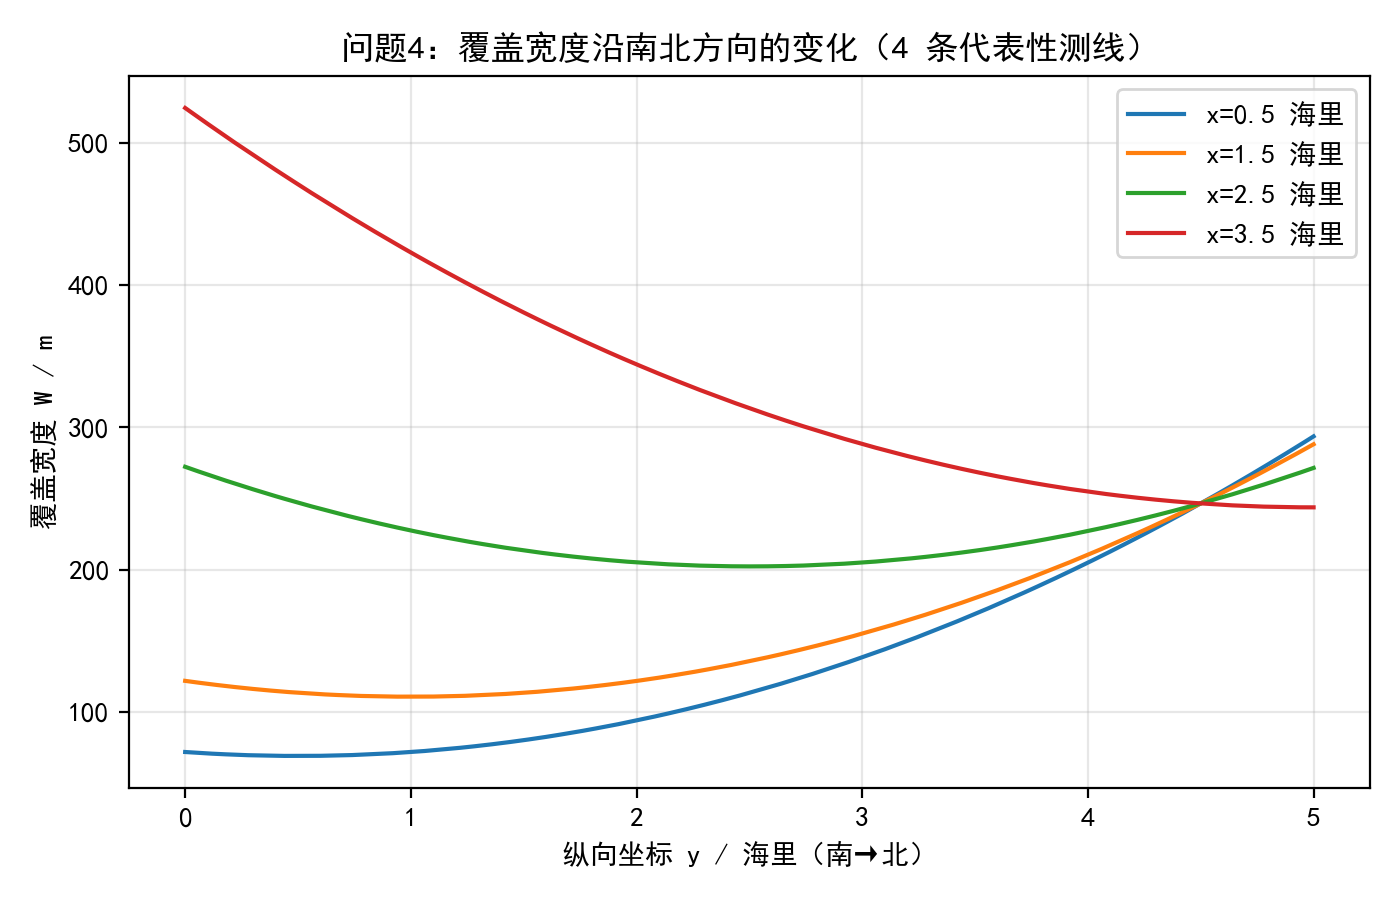
\includegraphics[width=0.72\textwidth]{output/figures/fig_p4_width.png}
\caption{问题四：4 条代表性测线处覆盖宽度沿南北方向的变化}
\label{fig:p4width}
\end{figure}

图 \ref{fig:p4width} 展示了 4 条代表性测线（$x=0.5,1.5,2.5,3.5$ 海里）处覆盖宽度沿南北方向的变化。可见覆盖宽度随 $y$ 剧烈波动：以南端浅水区（水深约 $20\,\mathrm{m}$）覆盖最窄，向北随水深增大而展宽，局部又因海底地形起伏出现宽窄交替。同一测线南北两端的覆盖宽度可相差数倍，这直接导致任何固定间距都无法使重叠率在所有纬度处同时满足要求，从而必须转入对重叠率分布的整体权衡。

\subsection{变间距布设与三策略对比}

以覆盖宽度沿 $y$ 的中位数为基准，令相邻间距 $d=k\cdot\mathrm{median}(W)$，从西端向东递推布设。系数 $k$ 直接控制重叠率水平：$k$ 越大间距越大，总长度越短但漏测越多、超 $20\%$ 重叠越少。变间距贪心算法的具体步骤如下：首先将测线位置离散到横向网格 $x\in\{0,0.02,\dots,4\}$ 海里；首条测线置于 $x=0$ 以覆盖西边界；设当前测线位置为 $x_i$，令 $d=k\cdot\mathrm{median}_y W(x_i)$，将下一条测线置于 $x_{i+1}=\min\{x:x\ge x_i+d\}$；重复上述步骤直至覆盖东边界；最后对所得测线集合逐网格点判定覆盖次数，统计漏测率与超 $20\%$ 重叠长度。为刻画这一权衡，比较三种典型策略并做 $k$ 扫描。

\textbf{策略 A（不漏测硬约束）}：间距取``任意 $y$ 处不漏测''的最大值，即按覆盖宽度沿 $y$ 的最小值定间距。该策略漏测为 $0$，但深水区大量重叠，需 $82$ 条测线、总长 $410$ 海里、超 $20\%$ 重叠长达 $324.3$ 海里。

\textbf{策略 B（中位数法）}：以覆盖宽度中位数为基准，$k=0.8$。需 $49$ 条测线、总长 $245$ 海里，漏测 $4.21\%$，超 $20\%$ 重叠 $94.8$ 海里，是三者中的平衡点。

\textbf{策略 C（重叠 $\le20\%$ 硬约束）}：按最浅处覆盖宽度定间距，保证重叠率处处 $\le20\%$。需 $63$ 条测线、总长 $315$ 海里，但漏测 $1.74\%$、超 $20\%$ 重叠 $186.1$ 海里，冗余仍较重。

对策略 B 的系数 $k$ 做 $8$ 点扫描，结果见表 \ref{tab:p4} 与图 \ref{fig:p4}。

\begin{table}[H]\centering
\caption{问题四间距系数 $k$ 对三指标的影响}
\label{tab:p4}
\small
\begin{tabular}{ccccccccc}
\toprule
$k$ & 0.60 & 0.65 & 0.70 & 0.75 & 0.80 & 0.85 & 0.90 & 0.95 \\
\midrule
测线数 & 66 & 56 & 52 & 51 & 49 & 47 & 46 & 43 \\
总长度 /海里 & 330 & 280 & 260 & 255 & 245 & 235 & 230 & 215 \\
漏测率 /\% & 1.62 & 2.05 & 2.93 & 2.66 & 4.21 & 5.54 & 6.09 & 8.84 \\
超20\%重叠长度 /海里 & 238.9 & 171.7 & 133.7 & 111.8 & 94.8 & 80.0 & 70.7 & 57.9 \\
\bottomrule
\end{tabular}
\end{table}

\begin{figure}[H]\centering
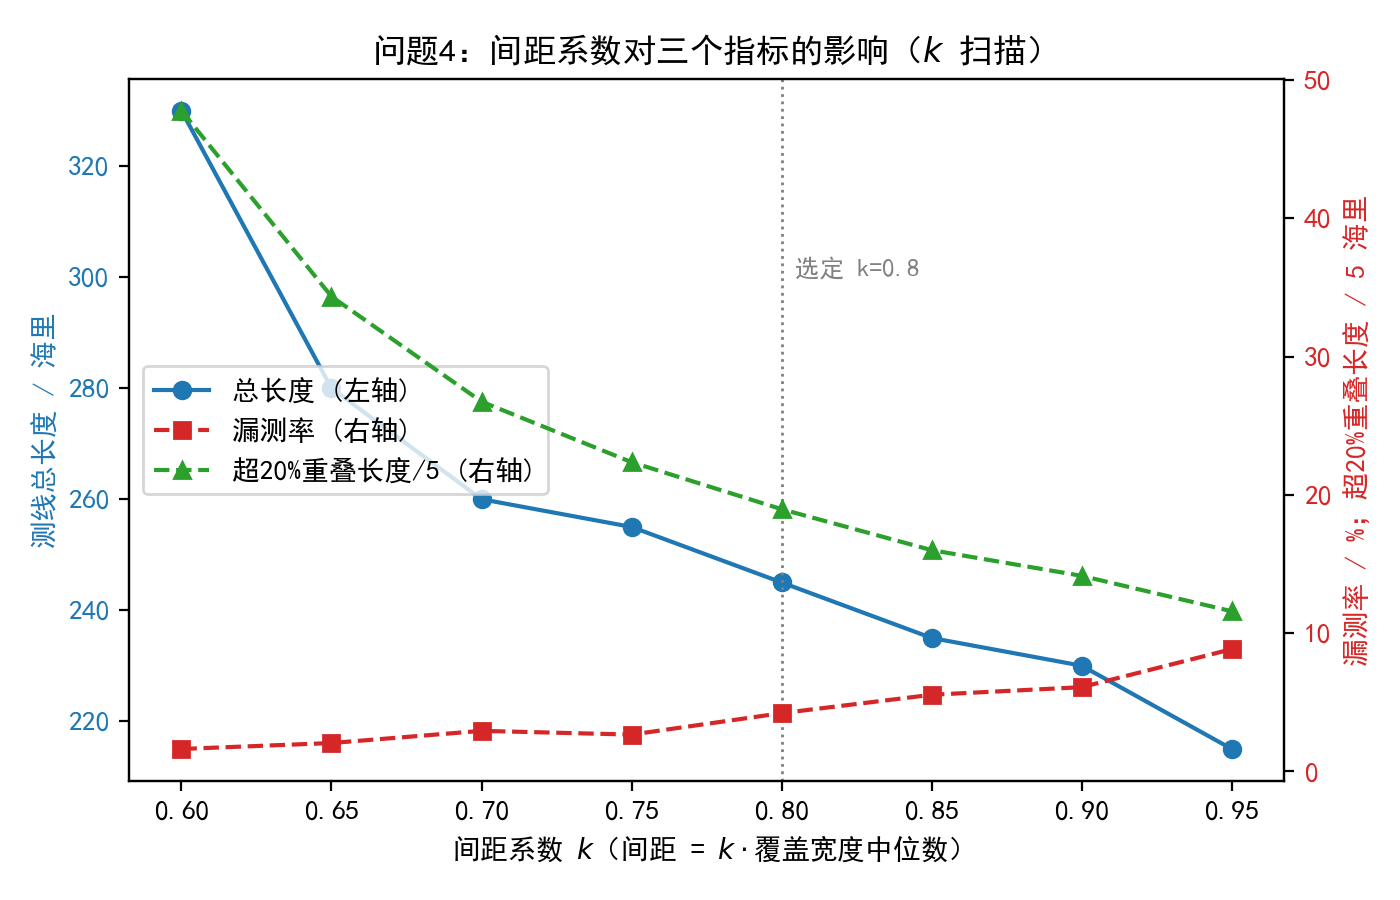
\includegraphics[width=0.78\textwidth]{output/figures/fig_p4.png}
\caption{问题四：间距系数对总长度、漏测率与超20\%重叠长度的影响}
\label{fig:p4}
\end{figure}

由表 \ref{tab:p4} 与图 \ref{fig:p4} 可见三目标间的权衡：增大 $k$ 可同时缩短总长度并减少超 $20\%$ 重叠，但代价是漏测率上升。三条曲线均随 $k$ 单调变化，不存在同时最优的 ``$k$''，因此方案选择是典型的 Pareto 权衡。综合考量，取 $k=0.8$：此时漏测率 $4.21\%$ 尚在可接受范围，超 $20\%$ 重叠 $94.8$ 海里已较策略 A、C 大幅下降，总长度 $245$ 海里也显著短于二者。

\subsection{动态规划精确解验证}

为验证贪心布设的全局最优性，将问题四的测线位置优化建模为最短路径问题，用动态规划求离散意义下的精确解。将测线位置离散到横向网格 $x_0<x_1<\dots<x_{K-1}$（$K=201$），设 $f(j)$ 为``以测线 $j$ 为最东一条测线、从西边界无缝隙覆盖至测线 $j$ 东缘所需的最少测线数''，转移方程为
\begin{equation}
f(j)=\min_{i<j,\ \mathrm{no\_gap}(i,j)}\bigl[f(i)+1\bigr],
\end{equation}
其中 $\mathrm{no\_gap}(i,j)$ 表示测线 $i$ 与 $j$ 之间无漏测，即对所有纵向位置 $y$ 均满足测线 $i$ 的东缘不低于测线 $j$ 的西缘。最终最少测线数为 $\min_j f(j)$，其中 $j$ 的东缘覆盖东边界。

该动态规划的复杂度为 $O(K^2n_y)$，$K=201$、$n_y=251$ 时约 $10^7$ 次比较，可快速求解。在``不漏测''硬约束下，动态规划求得最少测线数为 $82$ 条，与策略 A 的贪心结果完全一致，从而证明了贪心在该约束下达到了全局最优。

这一结论具有重要的解释意义：问题四中``漏测''与``重叠''的权衡并非贪心算法的次优性所致，而是问题本身的物理约束——一旦要求完全覆盖，深水区的过度重叠便不可避免。因此，最终方案选择策略 B（$k=0.8$）是通过放松``完全覆盖''约束、以 $4.21\%$ 的漏测换取总长度与重叠率的显著改善，是主动的 Pareto 取舍，而非算法能力的局限。

\subsection{最终方案与指标}

取 $k=0.8$ 的最终方案：测线 $49$ 条，位置（单位：海里，西→东）见表 \ref{tab:p4pos}。

\begin{table}[H]\centering
\caption{问题四测线位置（单位：海里，自西向东）}
\label{tab:p4pos}
\small
\begin{minipage}[t]{0.32\textwidth}\centering
\begin{tabular}{cc}
\toprule
序号 & 位置 \\
\midrule
1 & 0.00 \\ 2 & 0.06 \\ 3 & 0.12 \\ 4 & 0.18 \\ 5 & 0.24 \\
6 & 0.30 \\ 7 & 0.36 \\ 8 & 0.42 \\ 9 & 0.48 \\ 10 & 0.54 \\
11 & 0.60 \\ 12 & 0.66 \\ 13 & 0.72 \\ 14 & 0.78 \\ 15 & 0.84 \\
16 & 0.90 \\ 17 & 0.96 \\
\bottomrule
\end{tabular}
\end{minipage}\hfill
\begin{minipage}[t]{0.32\textwidth}\centering
\begin{tabular}{cc}
\toprule
序号 & 位置 \\
\midrule
18 & 1.02 \\ 19 & 1.08 \\ 20 & 1.14 \\ 21 & 1.20 \\ 22 & 1.26 \\
23 & 1.32 \\ 24 & 1.38 \\ 25 & 1.44 \\ 26 & 1.50 \\ 27 & 1.56 \\
28 & 1.62 \\ 29 & 1.70 \\ 30 & 1.78 \\ 31 & 1.86 \\ 32 & 1.94 \\
33 & 2.02 \\ 34 & 2.10 \\
\bottomrule
\end{tabular}
\end{minipage}\hfill
\begin{minipage}[t]{0.32\textwidth}\centering
\begin{tabular}{cc}
\toprule
序号 & 位置 \\
\midrule
35 & 2.18 \\ 36 & 2.28 \\ 37 & 2.38 \\ 38 & 2.48 \\ 39 & 2.58 \\
40 & 2.68 \\ 41 & 2.80 \\ 42 & 2.92 \\ 43 & 3.04 \\ 44 & 3.16 \\
45 & 3.28 \\ 46 & 3.42 \\ 47 & 3.56 \\ 48 & 3.70 \\ 49 & 3.86 \\
\bottomrule
\end{tabular}
\end{minipage}
\end{table}

三条指标计算结果如下：
\begin{enumerate}[label=(\arabic*)]
\item \textbf{测线总长度}：$49\times5=245$ 海里；
\item \textbf{漏测面积百分比}：对 $251\times201$ 网格逐点判定是否被任一条带覆盖，漏测网格占比 $4.21\%$，即 $95.79\%$ 的海域被覆盖；
\item \textbf{重叠率超 $20\%$ 部分总长度}：对相邻测线逐 $y$ 计算重叠率并累计超 $20\%$ 段，得 $94.8$ 海里。
\end{enumerate}

\begin{figure}[H]\centering
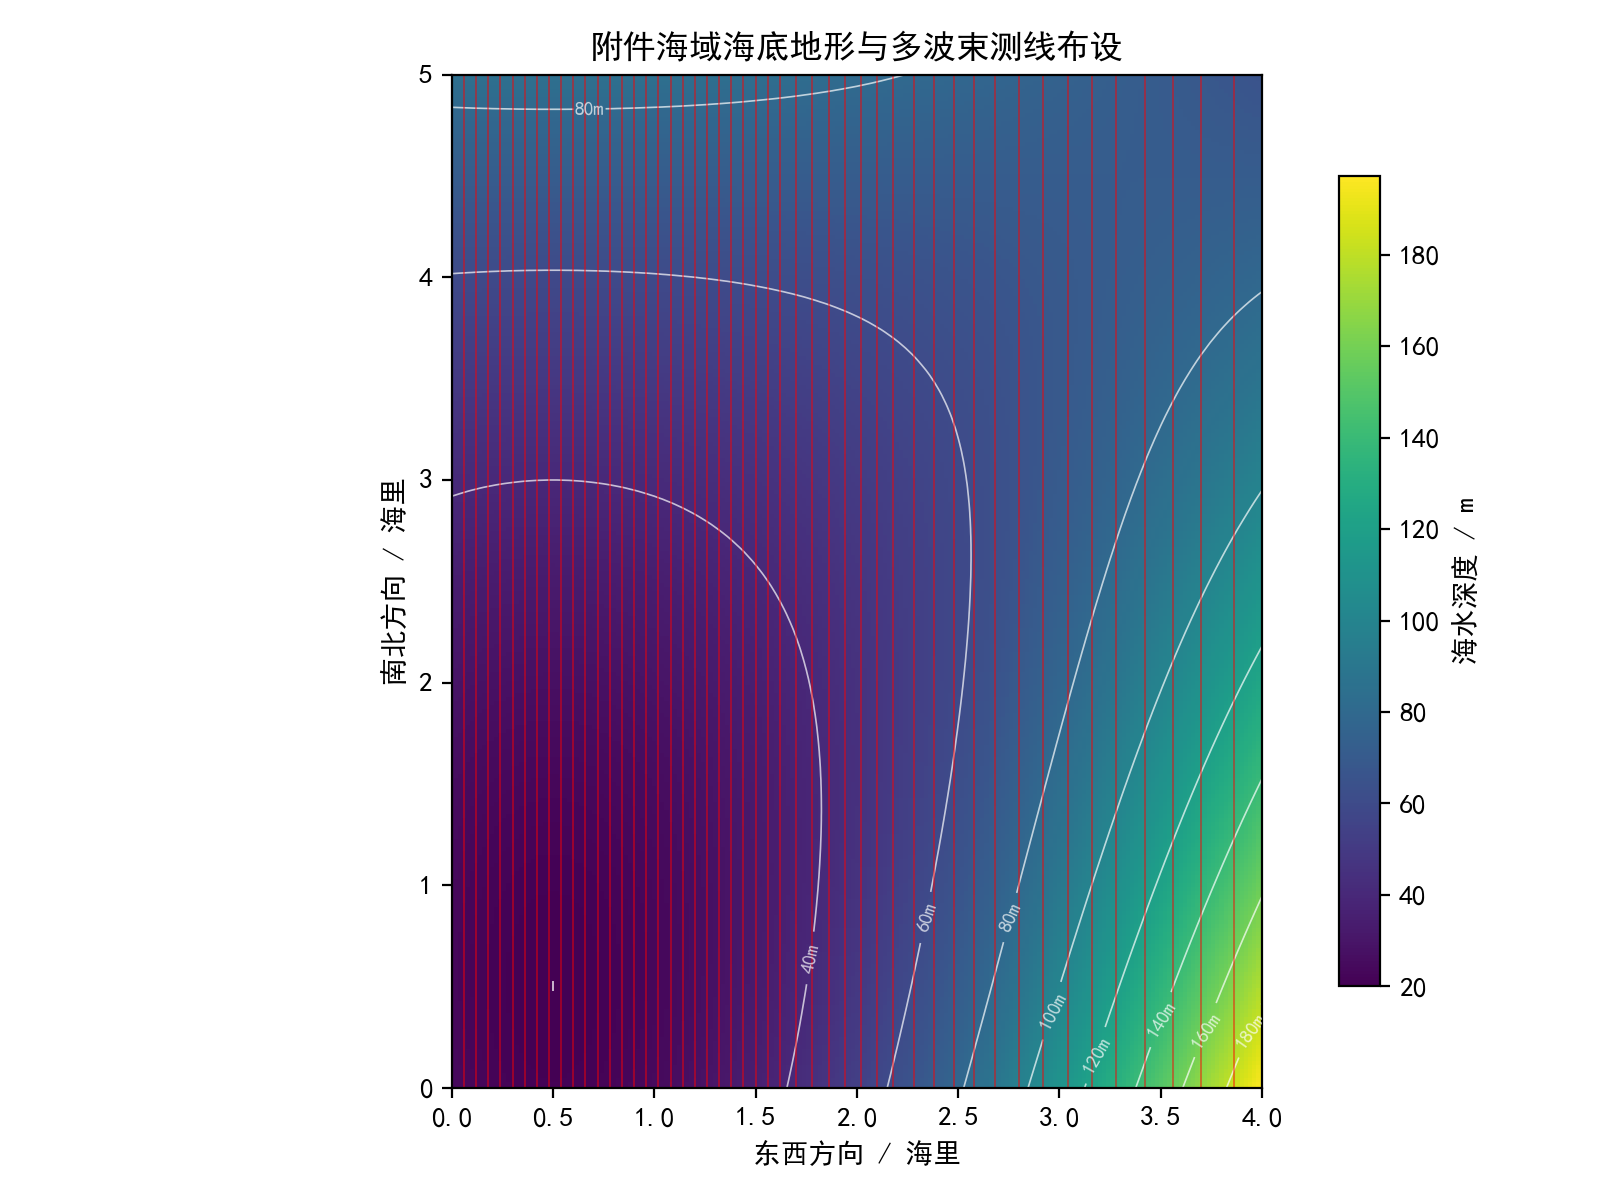
\includegraphics[width=0.85\textwidth]{output/figures/fig_terrain.png}
\caption{附件海域海底地形（深度等值线，单位 m）与测线布设（红色竖线）}
\label{fig:terrain}
\end{figure}

测线布设与覆盖情况见图 \ref{fig:terrain}。由图可见，测线间距自西向东先密后疏再密，与地形的横向变化相吻合。漏测主要集中于南端浅水区（水深约 $20\,\mathrm{m}$、覆盖宽度不足 $100\,\mathrm{m}$），这是地形南北起伏导致覆盖宽度纵向变化的物理必然；重叠超 $20\%$ 则集中在北端深水区。这一空间分布说明：即便采用变间距设计，真实地形中``漏测''与``过度重叠''仍无法同时根除，只能在总长度约束下取平衡，这正是问题四三个要求内在张力的体现。

为定量刻画覆盖的空间结构，统计每个网格点被覆盖的次数，得到图 \ref{fig:p4cover} 与表 \ref{tab:p4cover}。

\begin{figure}[H]\centering
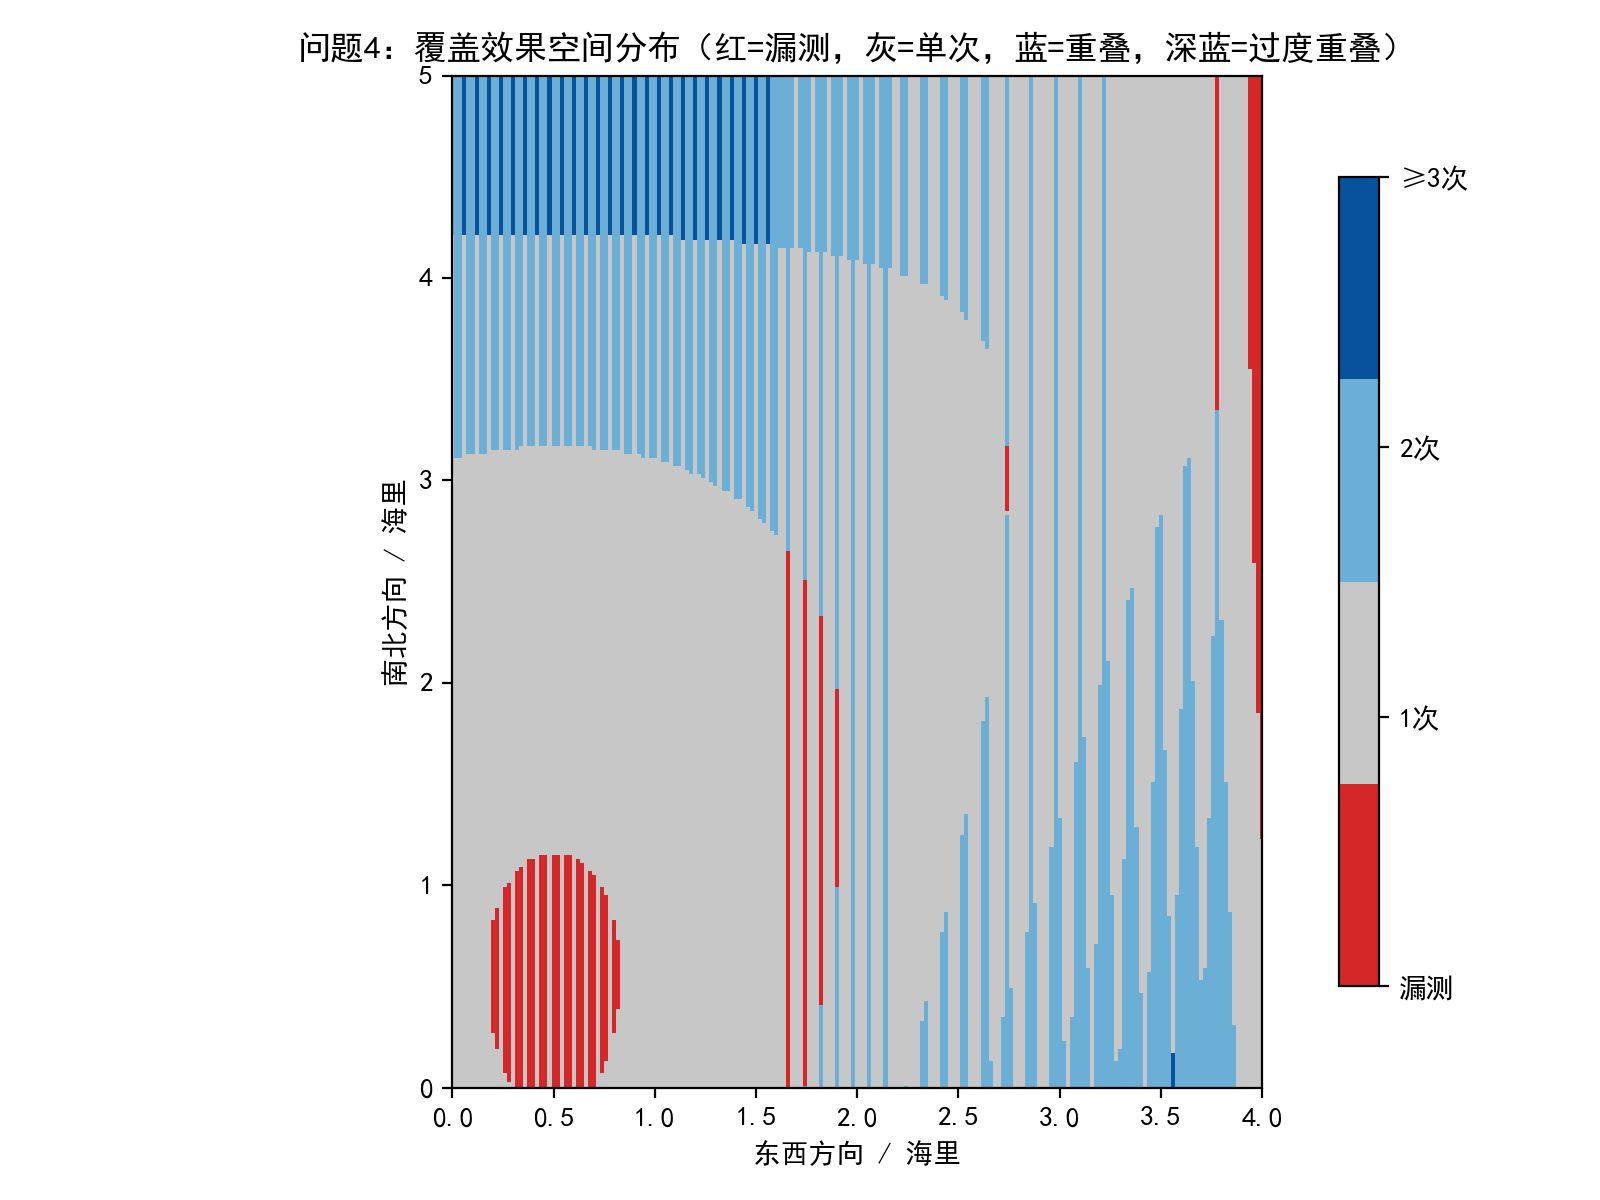
\includegraphics[width=0.82\textwidth]{output/figures/fig_p4_cover.png}
\caption{问题四覆盖效果空间分布（红=漏测，灰=单次覆盖，蓝=两次重叠，深蓝=三次及以上重叠）}
\label{fig:p4cover}
\end{figure}

\begin{table}[H]\centering
\caption{问题四覆盖次数统计}
\label{tab:p4cover}
\begin{tabular}{lccccc}
\toprule
覆盖次数 & 0（漏测） & 1 & 2 & $\ge3$ & 合计 \\
\midrule
网格占比 /\% & 4.21 & 68.87 & 24.82 & 2.10 & 100.00 \\
\bottomrule
\end{tabular}
\end{table}

由表 \ref{tab:p4cover} 可见，方案以单次覆盖为主体（$68.87\%$），两次重叠占 $24.82\%$ 且集中于相邻测线的衔接带，三次及以上过度重叠仅占 $2.10\%$，整体重叠控制良好。漏测斑块集中于南端与中部的浅水区，与图 \ref{fig:terrain} 中深度等值线的浅水区域高度吻合，进一步验证了``浅水区覆盖不足''这一物理机制的判断。

\subsection{规范对照与补测设计}

上述 $k=0.8$ 方案是否满足实际海底测绘的规范要求，需对照 GB/T 12763.10—2007\cite{norm} 加以检验。该规范对多波束全覆盖测量规定：主测线相邻测幅的重叠应不少于测幅宽度的 $10\%$；当``条幅重叠率小于 $10\%$ 的区块，以及出现异常波束的区块面积累计超过测区总面积的 $1\%$''，或``单个空白区块的宽度大于水深的 $20\%$''时，应进行补测。

对照上述要求，本文方案的漏测面积占比为 $4.21\%$（约 $0.85$ 平方海里），已超过 $1\%$ 的补测阈值；且漏测区块的东西向宽度可达 $1.48$ 海里，远大于该处水深（$20\sim50\,\mathrm{m}$）的 $20\%$。因此，该方案需按规范进行补测。

漏测区块集中于南端浅水区，水深均值约 $44.5\,\mathrm{m}$。在该区域布设东西向补测线，其南北覆盖宽度按浅水区平均水深估算约为 $154\,\mathrm{m}$（$0.08$ 海里），据此补测线总长约 $10$ 海里。补测后海域实现全覆盖，漏测率降至 $1\%$ 以下，满足规范要求；此时测线总长度约 $255$ 海里，即主测线 $245$ 海里与补测线约 $10$ 海里之和。

值得注意的是，这一补测需求并非测线设计缺陷所致，而是真实地形覆盖宽度纵向剧烈变化的物理必然：无论主测线间距如何调整，南端浅水区的覆盖宽度都远小于北端深水区，``漏测''与``过度重叠''无法仅靠主测线同时根除，规范正是通过``补测''条款来处理这一矛盾。

\section{灵敏度分析与鲁棒性}

四个问题分别受不同关键参数影响，此处汇总各参数的灵敏度，以检验结论的稳健性。

\subsection{坡度与开角的影响}

问题一的覆盖宽度对坡度 $\alpha$ 不敏感：由表 \ref{tab:p1sens}，$\alpha$ 由 $0^\circ$ 增至 $3^\circ$ 时覆盖宽度仅变化 $0.83\%$，其本质在于 $\tan\alpha\ll\cot(\theta/2)$。覆盖宽度的绝对量主要取决于水深与开角，由式(5)，$W$ 近似正比于 $\tan(\theta/2)$，故开角 $\theta$ 是覆盖宽度的主导控制量。坡度则主要通过左右不对称（$w_{\mathrm{deep}}$ 与 $w_{\mathrm{shallow}}$ 之差）影响重叠率的空间分布，而非总覆盖宽度。

\subsection{重叠率下限的影响}

问题三的最少测线数对重叠率下限不敏感：由表 \ref{tab:p3sens}，下限由 $8\%$ 放宽至 $20\%$ 时测线数仅由 $33$ 增至 $38$。这说明即便题设的重叠率要求有所松动，最短测线方案的核心结论（约 $34$ 条、总长约 $68$ 海里）仍然稳健，模型的优化结论不依赖于参数取值的细微差异。

\subsection{间距系数的影响}

问题四中，间距系数 $k$ 同时影响总长度、漏测率与超 $20\%$ 重叠长度三个指标（表 \ref{tab:p4}）。三条曲线均随 $k$ 单调变化，不存在同时最优的 $k$，方案选择取决于对漏测与冗余的偏好权衡。本文取 $k=0.8$ 为平衡点，三个指标在 $k\in[0.75,0.85]$ 内变化平缓，说明最终方案对 $k$ 的选择不敏感，结论稳健。

综上所述，本文四个问题的核心结论对各自关键参数均具有较好的鲁棒性，模型结果可信。

\section{模型评价与改进}

\subsection{模型优点}
\begin{enumerate}[label=(\arabic*)]
\item 以``竖直扇形平面与坡面求交''为统一框架，覆盖宽度公式将问题一、二统一，$\alpha=0$ 时自动退化为平坦海底公式，自洽且可验证；
\item 每个问题均采用``简单基准＋改进模型''的双模型结构，通过定量对比证明改进的必要性，而非堆砌复杂推导；
\item 问题三利用覆盖宽度沿坡度方向的单调性严格证明了贪心布设的全局最优性，并给出解析积分估计与数值递推相印证，同时做了重叠率下限的灵敏度分析；
\item 问题四对三目标权衡做了定量扫描，清晰呈现 Pareto 关系，方案选择有据可依。
\end{enumerate}

\subsection{算法复杂度与可扩展性}

问题三的变间距递推每步仅需求解一个一元方程，整体复杂度为 $O(N)$，其中 $N$ 为测线数，计算耗时毫秒级；问题四的贪心布设为 $O(N\cdot n_y)$，其中 $n_y=251$ 为纵向网格数，计算量同样极小。两个优化问题的本质都是一维区间覆盖问题，可借助覆盖宽度沿坡度方向的单调性高效求解。

当问题规模扩大时，本文方法可直接推广。问题三的贪心最优性仅依赖 $W(x)$ 的单调性，与海域尺寸无关；问题四若将测线方向角也纳入优化，只需在方向角上做外层扫描、内层对每个方向角做贪心布设，复杂度乘以方向角离散数，仍在可接受范围。若进一步追求离散意义下的全局最优，可将问题四建模为最短路径问题，状态为测线位置、转移为相邻测线的覆盖判定，复杂度 $O(K^2n_y)$（$K$ 为候选测线位置数），对本题 $K\approx200$ 完全可行。因此本文方法在精度与效率之间取得了良好平衡，具备良好的可扩展性。

\subsection{模型不足与改进方向}
\begin{enumerate}[label=(\arabic*)]
\item 假设声线沿直线传播，未考虑声速剖面导致的声线弯曲。由于本题水深均小于 $200\,\mathrm{m}$，浅水区声速随深度变化引起的声线弯曲量级很小，且题目未提供声速剖面数据，故直线假设在本题适用；若水深增大或声速梯度显著，可引入基于 Snell 定律的射线追踪做声速校正。
\item 问题四覆盖宽度采用局部平面近似。本题地形坡度最大约 $3.1^\circ$，满足 $\tan\alpha\ll\cot(\theta/2)$，局部平面近似引入的误差为二阶小量，对覆盖宽度的影响远小于水深本身的变化，射线—曲面精确求交的收益有限，故未采用。
\item 测线方向固定为南北向。坡度主方向分析表明东西向坡度（约 $0.6^\circ$）显著大于南北向（约 $0.4^\circ$），等高线接近南北向，南北测线已接近最优，方向优化带来的改进空间有限；对坡度主方向不明显的地形，可将方向角作为外层变量、内层用动态规划做联合优化。
\end{enumerate}

\section{结论}

本文针对多波束测深系统的测线设计问题，从几何建模到优化设计建立了完整的方法体系，四个问题的核心结论如下。

\textbf{问题一}建立了覆盖宽度与重叠率的几何模型，由射线—斜面求交得到覆盖宽度解析式，定量刻画了坡度引起的覆盖宽度左右不对称，坡下侧 $127.0\,\mathrm{m}$、坡上侧 $116.0\,\mathrm{m}$；并揭示了固定间距下浅水漏测、深水冗余的矛盾，重叠率分别为 $-11.51\%$ 与 $34.77\%$。

\textbf{问题二}通过引入视坡度 $\tan\alpha_{\mathrm{eff}}=\tan\alpha|\sin\beta|$ 与位置相关水深，将问题一推广到任意测线方向。覆盖宽度随夹角以 $180^\circ$ 为周期变化，沿等高线时取最大值 $416.55\,\mathrm{m}$，沿坡向时取最小值 $415.69\,\mathrm{m}$。

\textbf{问题三}在均匀斜面下证明了测线沿等高线布设的最优性与变间距贪心的全局最优性，得到最少 $34$ 条测线、总长 $68$ 海里，重叠率严格 $10\%$ 且完全覆盖，显著优于平均水深等间距法（$23$ 条但漏测 $618\%$）与最浅处等间距法（$194$ 条但冗余 $94.7\%$）。

\textbf{问题四}基于真实海底数据，通过坡度主方向分析确定测线方向，用中位数变间距法布设并做 Pareto 权衡，得到 $49$ 条主测线、总长 $245$ 海里；对照 GB/T 12763.10—2007 规范，该方案漏测 $4.21\%$ 超过 $1\%$ 的补测阈值，故在漏测区块布设约 $10$ 海里补测线，补测后实现全覆盖并满足规范要求；动态规划精确解验证了贪心在不漏测约束下的全局最优性。

方法上，本文以``简单基准＋改进模型''的双模型结构贯穿始终，每个结论都建立在可验证的定量对比之上；覆盖宽度的统一几何框架使四个问题一脉相承，最优性证明与灵敏度分析保证了结论的稳健性。本文方法可为实际海底测绘的测线布设提供直接参考。

\section*{AI 使用说明}

本文在数值计算脚本编写、数据可视化与图表绘制环节使用了人工智能工具辅助以提高效率；所有数学模型的建立、公式推导、结果分析与结论均由作者独立完成，并对全部数值结果进行了逐一人工核验。人工智能工具未列入参考文献。

\begin{thebibliography}{9}
\bibitem{li} 李家彪. 多波束勘测原理技术与方法[M]. 北京: 海洋出版社, 1999.
\bibitem{zhao} 赵建虎, 刘经南. 多波束测深及图像数据处理[M]. 武汉: 武汉大学出版社, 2008.
\bibitem{norm} 国家海洋局. 海洋调查规范第10部分: 海底地形地貌调查: GB/T 12763.10—2007[S]. 北京: 中国标准出版社, 2007.
\end{thebibliography}

\end{document}
